\documentclass{../tikzfig}

\begin{document}
	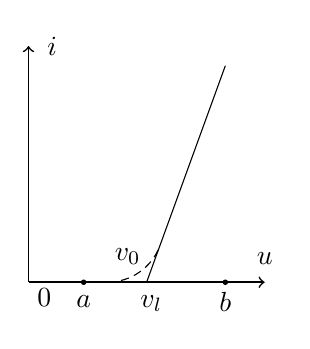
\begin{tikzpicture}
		\draw[->, semithick] (0,0) -- (0,3);
		\draw[->, semithick] (0,0) -- (3,0);
		\node[draw=none] at (0.3,3) {$i$};
		\node[draw=none] (node1) at (3,0.3
		) {$u$};
		\node[draw=none] at (0.2,-0.2) {0};
		% Точка a
		\def\xa{0.7}
		\node[draw=none] at (\xa,-0.25) {$a$};
		\fill (\xa,0) circle (1pt);
		
		% Точка b
		\def\xb{2.5}
		\node[draw=none] at (\xb,-0.25) {$b$};
		\fill (\xb,0) circle (1pt);
		
		\draw (1.5,0) -- (\xb,2.75);
		
		\draw[densely dashed] (1,0) arc (270:340:0.715cm);
		\node[draw=none] at (1.26,0.33) {$v_0$};
		\node[draw=none] at (1.56,-0.27) {$v_l$};
	\end{tikzpicture}
\end{document}